%% Template article for Elsevier's document class `elsarticle'
%% with numbered style bibliographic references
%% SP 2008/03/01
%%
%%
%%
%% $Id: elsarticle-template-num.tex 4 2009-10-24 08:22:58Z rishi $
%%
%%
\documentclass[preprint,12pt]{elsarticle}
%% Use the option review to obtain double line spacing
%% \documentclass[preprint,review,12pt]{elsarticle}
%% Use the options 1p,twocolumn; 3p; 3p,twocolumn; 5p; or 5p,twocolumn
%% for a journal layout:
%% \documentclass[final,1p,times]{elsarticle}
%% \documentclass[final,1p,times,twocolumn]{elsarticle}
%% \documentclass[final,3p,times]{elsarticle}
%% \documentclass[final,3p,times,twocolumn]{elsarticle}
%% \documentclass[final,5p,times]{elsarticle}
%% \documentclass[final,5p,times,twocolumn]{elsarticle}

%% if you use PostScript figures in your article
%% use the graphics package for simple commands
%% \usepackage{graphics}
%% or use the graphicx package for more complicated commands
%\usepackage{graphicx}
%% or use the epsfig package if you prefer to use the old commands
%% \usepackage{epsfig}

%% The amssymb package provides various useful mathematical symbols
%\usepackage{amssymb}
%% The amsthm package provides extended theorem environments
%% \usepackage{amsthm}

% custom packages
\usepackage[nolist]{acronym}
\usepackage{amsmath,amsfonts,amssymb,amsthm}
\usepackage{natbib}
\usepackage[colorlinks=false]{hyperref}
\usepackage{graphicx,hypernat}
\usepackage{geometry}
\usepackage{color}
\usepackage{multirow}
\usepackage{booktabs}
\usepackage{rotating}
%% The lineno packages adds line numbers. Start line numbering with
%% \begin{linenumbers}, end it with \end{linenumbers}. Or switch it on
%% for the whole article with \linenumbers after \end{frontmatter}.
%% \usepackage{lineno}

%% natbib.sty is loaded by default. However, natbib options can be
%% provided with \biboptions{...} command. Following options are
%% valid:

%%   round  -  round parentheses are used (default)
%%   square -  square brackets are used   [option]
%%   curly  -  curly braces are used      {option}
%%   angle  -  angle brackets are used    <option>
%%   semicolon  -  multiple citations separated by semi-colon
%%   colon  - same as semicolon, an earlier confusion
%%   comma  -  separated by comma
%%   numbers-  selects numerical citations
%%   super  -  numerical citations as superscripts
%%   sort   -  sorts multiple citations according to order in ref. list
%%   sort&compress   -  like sort, but also compresses numerical citations
%%   compress - compresses without sorting
%%
%% \biboptions{comma,round}
% \biboptions{}
\journal{Robotics and Autonomous System}
\begin{document}
%%
\begin{acronym}
%==== A B C D ====
\acro{AFM}{attractive field model}
\acro{AGV}{automated guided vehicle}
\acro{APCD}{average production completion delay}
\acro{APMW}{average pending maintenance work-load}
%\acro{AS}{active space}
\acro{BMS}{biology-inspired manufacturing system}
\acro{CCD}{charge-coupled device}
%\acro{CCM}{centralized communication mode}
\acro{DEM}{data and event management}
\acro{DOL}{division of labour}
%==== E F G H ====
%\acro{EPSRC}{Engineering and Physical Sciences Research Council}
\acro{GigE}{Gigabyte Ethernet}
\acro{GIL}{Global Interpreter Lock}
%\acro{GPS}{global positioning system}	
\acro{GSNC}{global sensing - no communication}
%\acro{GUI}{graphical user interface}
\acro{HEAD}{hybrid event-driven architecture on D-Bus}
%====  I J K L ====
%\acro{IF}{independent founders}
%\acro{INS}{indoor navigation system}
\acro{IPC}{inter-process communication}
%\acro{IR}{infrared}
%\acro{LCM}{local communication mode}
\acro{LSLC}{local sensing - local communication}
%==== M N O P ====
\acro{MOM}{maintenance only mode}
\acro{MRS}{multi-robot system}
\acro{MRTA}{multi-robot task allocation}
\acro{P2P}{peer-to-peer}
%\acro{PF}{potential field}
\acro{PMM}{production and maintenance mode}
%=====  Q R S T ====
\acro{RCC}{robot-controller client}
%\acro{RW}{random walk}
\acro{SDK}{software-development kit}
%\acro{SF}{swarm founders}
\acro{SHM}{shared memory}
%\acro{SI}{swam intelligence}
%\acro{SO}{self-organization}
%\acro{SR}{self-regulation}
%\acro{SRS}{swarm robotic system}
\acro{TPS}{task perception server}
%==== U V W X ====
%==== Y Z ==== 
\end{acronym}
\begin{frontmatter}
%%
%% Title, authors and addresses
%%
%% use the tnoteref command within \title for footnotes;
%% use the tnotetext command for the associated footnote;
%% use the fnref command within \author or \address for footnotes;
%% use the fntext command for the associated footnote;
%% use the corref command within \author for corresponding author footnotes;
%% use the cortext command for the associated footnote;
%% use the ead command for the email address,
%% and the form \ead[url] for the home page:
%%
%% \title{Title\tnoteref{label1}}
%% \tnotetext[label1]{}
%% \author{Name\corref{cor1}\fnref{label2}}
%% \ead{email address}
%% \ead[url]{home page}
%% \fntext[label2]{}
%% \cortext[cor1]{}
%% \address{Address\fnref{label3}}
%% \fntext[label3]{}
%%
\title{Self-regulated Multi-robot Task~Allocation:\\ A Taxonomy and Comparison of Centralized and Local Communication Strategies}
%%
%% use optional labels to link authors explicitly to addresses:
\author[label1]{Md Omar Faruque Sarker and Torbj{\o}rn S. Dahl}
\address[label1]{Cognitive Robotics Research Centre\\
Newport Business School,
Allt-yr-yn Campus\\ %Allt-yr-yn Avenue\\
Newport, NP20 5DA,
United Kingdom.\\
Mdomarfaruque.Sarker \vline Torbjorn.Dahl@newport.ac.uk}
%\address[label1]{<address>}
%
%\author{}
%
%\address{}
%
\begin{abstract}
This paper proposes to solve the MRTA problem using a set of previously published generic rules for division of labour derived from the observation of ant, human and robotic social systems. The concrete form of these rules, the \textit{attractive filed model} (AFM), provides sufficient abstraction to local communication and sensing which is uncommon in existing MRTA solutions. We have validated the effectiveness of AFM to address MRTA  using two bio-inspired communication and sensing strategies: ``global sensing - no communication'' and ``local sensing - local communication''. The former is realized using a centralized communication system and the latter is emulated under a peer-to-peer local communication scheme. They are applied in a  manufacturing shop-floor scenario using 16 e-puck robots. A flexible multi-robot control architecture, \textit{hybrid event-driven architecture on D-Bus}, has been outlined which uses the state-of-the-art D-Bus interprocess communication.  Based-on the organization of task-allocation, communication and interaction among robots, a  novel taxonomy of MRTA solutions has been proposed to remove the ambiguities found in existing MRTA solutions. Besides, a set of domain-independent metrics, e.g., plasticity, task-specialization and energy usage, has been formalized to compare the performances of the above two strategies.
\end{abstract}
%%
\begin{keyword}
multi-robot system \sep multi-robot task allocation
%% keywords here, in the form: keyword \sep keyword
%% MSC codes here, in the form: \MSC code \sep code
%% or \MSC[2008] code \sep code (2000 is the default)
\end{keyword}
%%
\end{frontmatter}
%%
%%
%% Start line numbering here if you want
%%
% \linenumbers
%%==================================================================
%% main text
\section{Introduction}
\label{sec:intro}
%%
%% [MRTA problem at a glance]
%-------------------------------
 Multi-robot systems can provide improved performance, fault-tolerance and robustness in complex and distributed tasks through parallelism and redundancy \cite{Arkin1998,Parker+2006}. However in order to get potential benefits of \aclp{MRS}, we need to answer a common research question. \textit{How can we allocate tasks among multiple robots dynamically?} Traditionally, this issue has been identified as the \acfi{MRTA} \cite{Gerkey+2004}. This issue can be treated as the \acfi{DOL} among robots, analogous to the DOL in biological and human social systems\footnote{Although the term ``division of labour'' is often used in biological literature and the term ``task-allocation'' is primarily used in multi-agent literature,  in this paper we have used these terms interchangeably.} \cite{Sendova-Franks+1999}.

MRTA is generally identified as the question of assigning tasks in an appropriate time to the appropriate robots considering the changes of the environment and/or the performance of other team members \cite{Gerkey+2003}. This is a {\em NP-hard} optimal assignment problem where optimum solutions can not be found quickly for large and complex problems \cite{Parker2008}.The complexities of the distributed MRTA problem arise from the fact that there is no central planner or coordinator for task assignments, and in a large \acl{MRS}, generally robots have limited capabilities to sense, to communicate and to interact locally. None of them has the complete knowledge of the past, present or future actions of other robots.

Early research on predefined task-allocation was dominated by intentional coordination \cite{Parker2008}, use of dynamic role assignment \cite{Chaimowicz2002} and market-based bidding approach \cite{Dias+2006}. Under these approaches, robots use direct task-allocation method, often to communicate with group members for negotiating on tasks. These approaches are intuitive, comparatively straight forward to design and implement and can be analysed formally. However, these approaches typically works well only when the number of robots are small ($\leq 10$) \cite{Lerman+2006}.

On the other hand, self-organized task-allocation approach relies on the emergent group behaviours, such as emergent cooperation \cite{Kube+1993}, adaptation rules \cite{Liu+2007} etc. They are more robust and scalable to large team sizes. However, most of the robotic researchers found that self-organized task-allocation approach is difficult to design, to analyse (formally) and to implement in real robots. The solutions from these systems are also sub-optimal. It is also difficult to predict exact behaviours of robots and overall system performance.

Within the context of the Engineering and Physical Sciences Research Council (EPSRC) project, ``Defying the Rules: How Self-regulatory Systems Work'', we have proposed to solve the above mentioned self-regulated DOL problem in an alternate way \cite{Arcaute+2008}. Our approach is inspired from the studies of emergence of task-allocation in both biological and human social systems. We have proposed four generic rules to explain self-regulation in those social systems. These four rules are: \textit{continuous flow of information}, \textit{concurrency}, \textit{learning} and \textit{forgetting}, all of them will be explained later. Primarily these rules deal with the issue of deriving local control laws for regulating an individual's task-allocation behaviour that can facilitate the DOL in the entire group. In order to  employ these rules in the individual level, we have developed a formal model of self-regulated DOL, called the \acfi{AFM}.

In biological social systems, communications among the group members, as well as sensing the task-in-progress, are two key components of self-organized DOL. In robotics, existing self-organized task-allocation methods rely heavily upon local sensing and local communication of individuals for achieving self-organized task-allocation. However, AFM differs significantly in this point by avoiding the strong dependence on the local communications and interactions found in many existing approaches to MRTA. AFM provides a rich abstraction to this requirement through a system-wide continuous flow of information about tasks, agent states etc. This flow of information can be achieved by using both centralized and decentralized communication modes under explicit and implicit communication strategies.

In order to enable continuous flow of information in our \acl{MRS}, we have implemented two types of sensing and communication strategies inspired by the self-regulated DOL found in two types of social wasps: {\em polistes} and {\em polybia} \cite{Jeanne1999}. Depending on the group size, these species follow different strategies for communication and sensing of tasks. Polistes wasps are called the {\em independent founders} in which reproductive females establish colonies alone or in small groups (in the order of $10^2$), but independent of any sterile workers. On the other hand, polybia wasps are called the {\em swarm founders} where a swarm of workers and queens initiate colonies consisting of several hundreds to millions of individuals.

The most notable difference in the organization of work of these two social wasps is: independent founders do not rely on any cooperative task performance while swarm founders interact with each-other locally to accomplish their tasks. The work mode of independent founders can be considered as {\em global sensing - no communication (GSNC)} where the individuals sense the task requirements throughout a small colony and do these tasks without communicating with each other. On the other hand, the work mode of swarm founders can be treated as {\em local sensing - local communication (LSLC)} where the individuals can only sense tasks locally due to large colony-size and they can communicate locally to exchange information, e.g. task-requirements (although their exact mechanism is unknown).In this study, we have used these two sensing and communication strategies to compare the performance of the self-regulated DOL of our robots under AFM. 

The main contributions of this paper are as follows:
\begin{itemize}
\item Interpretation of AFM, an inter-disciplinary generic model of division of labour, as a basic mechanism of self-regulated MRTA.
\item Validation of the model through experiments with reasonably large number of real robots i.e., 16 e-puck robots.
\item Comparisons of the performances of two bio-inspired sensing and communication strategies in achieving self-regulated MRTA.
\item Development of a flexible multi-robot control architecture using D-Bus inter-process communication technology.
\item Classification of MRTA solutions based on three major axes: organization of task-allocation, interaction and communication.
\end{itemize}
%%===================================================================
\section{Related work}
\label{sec:bg}
%%
\begin{figure}
\centering
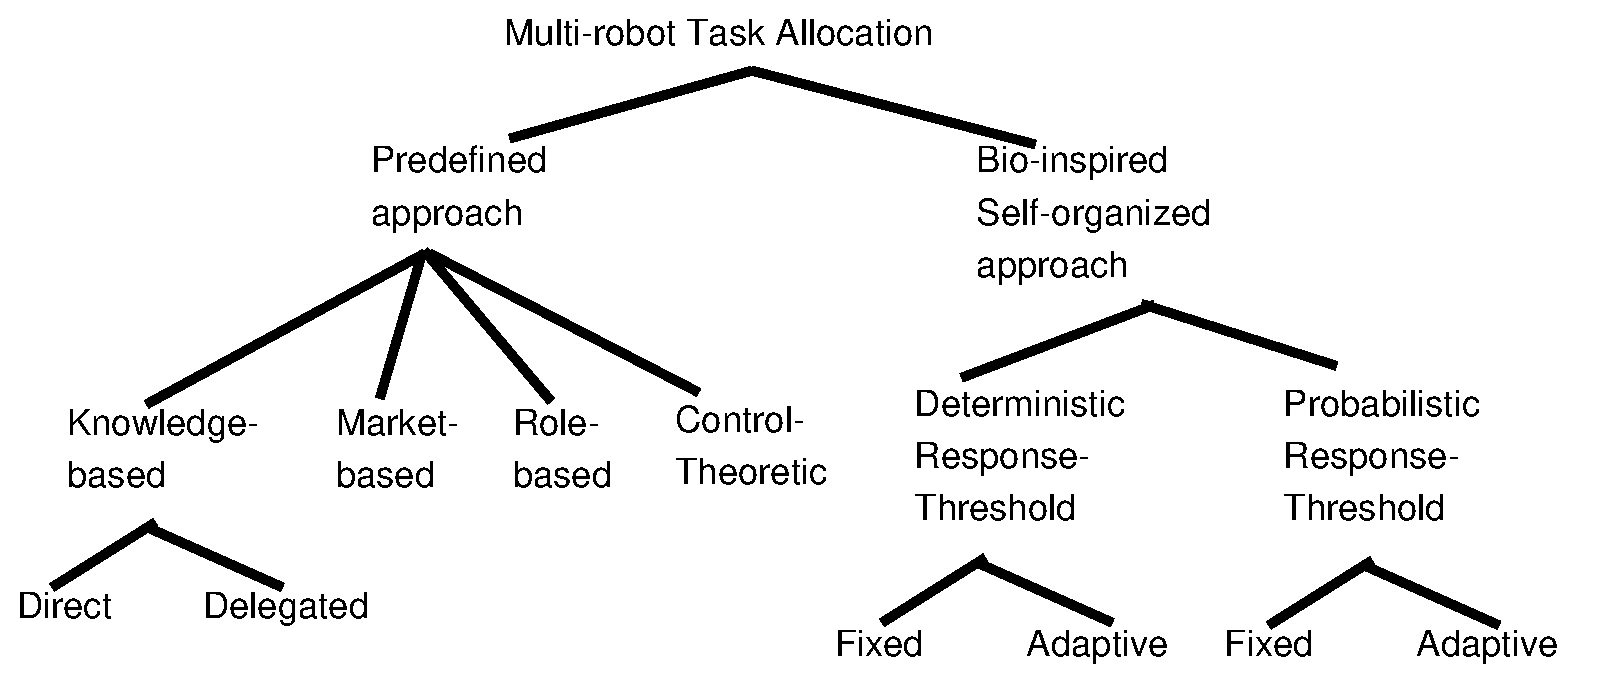
\includegraphics[width=12cm, angle=0]
{./images/ta-categories.eps}
\caption{\small Classification of MRTA solutions.}
\label{fig:mrta-classification} % Give a unique label
\end{figure}
%%
Since 90s, MRTA many robot control architectures   have been solely designed to address MRTA issue from different perspectives. Based-on the high-level design of those solutions, here we have classified them into two major categories: 1) predefined or intentional task-allocation and 2) bio-inspired self-organized task-allocation. Fig. \ref{fig:mrta-classification} illustrates our classification.

In most of the traditional multi-robot system, task allocation is done using well-defined models of tasks and environments. Here it is assumed that the system designer has the precise knowledge about tasks, robot-capabilities etc. Many flavours of the type of task-allocation can be found in the literature. Knowledge-based and multi-agent based approaches use various knowledge-based techniques to represent tasks, robot capabilities etc. One of the early well-known MRTA architecture of this category was ALLIANCE  in which each robot models the ability of team-members to perform tasks by observing their current task performances and collecting relevant task quality statistics e.g. time to complete tasks \cite{Parker1998}. Robots use these models to select a task that benefit  the group as a whole. 

Similar to  ALLIANCE, multi-agent based task allocation also  use both centralized and decentralized approaches for allocating tasks among  its  peers. \citet{Shen+2001} presented a detailed categorization where in a multi-agent system task allocation can be done by using various agents ranging from a central supervising agent or a few mediator agents to  all independent agents. 

As a feasible alternative to the above common multi-agent based task-allocation techniques, many researchers have been following the market-based bidding approach \citet{Dias+2006}. Originated from the Contract-Net Protocol, market-based approach can be implemented as a centralized auctioning system or as a combination of {\em a few auctioneers -- all bidders} or, independently {\em all auctioneers -- all bidders}. For example, in a completely distributed system, when a robot needs to perform a task for which it does not have necessary expertise or resources, it broadcasts a task-announcement message, often with  a expiry time of that message. Robots, that received the message and can perform that task, return a bid message. The initiating robot or {\em  manager} selects one (or more) bidder, called as {\em contractor}, and offers the opportunity to complete the task. The choice of contractor is done by the manager with a mutual agreement with contractor that maximizes the individual profits.

Under role or value-based task-allocation scheme, each role assumes several specific tasks and each robot selects roles that best suit their individual skills and capabilities \cite{Chaimowicz2002}. In this case, robots are typically heterogeneous, each one having variety of different sensing, computation and effector capabilities. Here robot-robot or robot-environment interactions are designed as a part of the organization. In multi-robot soccer \cite{Stone+1999}, positions played by different  robots are often defined as roles, e.g. goal-keeper, left/right defender, left/right forwarder etc. 

Under control-theoretic approaches, a model of the system is usually developed that converts the task specification into an objective function to be optimized. This model typically  uses  the rigid  body dynamics of the robots assuming the masses and other parameters well-known. Control laws of individual robots are derived either by analytically or by run-time iterations. Unlike most other approaches where task-allocation problem is taken as discrete, control-theoretic approaches can produce continuous  solutions. The formalisms of these systems allow system designer to check the system's controllability, stability and related other properties.  These systems typically use some degree of centralization, e.g. choosing a leader robot.  Example of control-theoretic approach include: multi-robot formation control \cite{Belta+2004}, multi-robot box-pushing \cite{Pereira+2003}  etc.

Predefined task-allocation through few other approaches are also present in the literature. For example, inspired by the vacancy chain phenomena in nature, \citet{Dahl+2004} proposed a vacancy chain scheduling algorithm for a restricted class of MRTA problems in spatially classifiable domains.

Task performance in self-organized approaches relies on the collective behaviours resulted from the local interactions of many simple and mostly homogeneous (or interchangeable) agents. Robots choose their tasks independently using the principles of self-organization, e.g. positive and negative feedback mechanisms, randomness. Moreover interaction among individuals and their environment are modulated by the stigmergic, local and broadcast communications.  Among many variants of self-organized task-allocation, most common type is threshold-based task-allocation \cite{Bonabeau+1999}. In this approach, a robot's decision to select a particular task depends largely on its perception of stimulus (demand for a task) and its corresponding response threshold for that task. 

Under deterministic response-threshold approach, each robot has a fixed or deterministic activation threshold for each task that needs to be performed. It continuously perceives or monitors the stimulus of all tasks that reflect the relative urgencies of tasks. When a particular task-stimuli exceeds a predefined  threshold the robot starts working on that task and gradually decreases this stimuli. When the task-stimuli falls below the fixed threshold the robot abandons that task. This type of approach has been effectively applied in foraging \cite{Krieger+2000,Liu+2007}, aggregation \cite{Agassounon+2002}. This fixed response-threshold can initially be same for all robots \cite{Jones+200}, or they can be different according robot capabilities or configuration of the system \cite{Krieger+2000}. Adaptive response threshold model changes or adapts the threshold over time. Response-threshold decreases often due to performance of a task and this enables a robot  to select that particular task more frequently or in other words it learns about that task \cite{Bonabeau+1999,Agassounon+2002}. 

Unlike deterministic approach, where robots always respond to a task-stimuli that has a largest stimulus above the threshold,  probabilistic approach offers a selection process based-on a probability distribution. Robots  always have small nonzero probabilities  for all tasks.

Most predefined task-allocation solutions are proposed within the context of a known or controlled environment where the modelling of tasks, robots, environments etc. becomes feasible. Note that here tasks can be arbitrarily complex that often require relatively higher sensory and processing abilities of robots. Robot-team can be consists of homogeneous or heterogeneous individuals, having different capabilities based on the variations in their hardware, software etc. But the uncertainty of the environment is assumed to be minimum. 

On the other hand, bio-inspired self-organized MRTA solutions are free from extensive modelling of environment, tasks or robot capabilities. Most of the existing research considers very simple form of one global task e.g. foraging, area cleaning, box-pushing etc. This is due to the fact that major focus of this approach is limited mainly to design individual robot controllers in such a way that a few simple  or {\em specific} tasks can be accomplished. More research is needed to verify the capabilities of self-organized approach in doing multiple complex tasks. At this moment, the bottom line remains as ``select simple robots for simple tasks (self-organized approach) and complex robots for complex tasks (predefined approach)''.

Both of the above task-allocation approaches expose their relative strengths and weaknesses when they are put under real-time experiments with variable number of robots and dynamic tasks. In an arbitrary event handling domain, \citet{kalra+2007}  compared between self-organized and predefined market-based task-allocation,  where they found that predefined  task-allocation was more efficient when the information was accurate, but threshold-based  approach offered similar quality of allocation at a fraction of cost  under noisy environment.  

\citet{Gerkey+2003} presented a comparative study of  the complexity and optimality of key architectures, e.g.  ALLIANCE \cite{Parker1998}, BLE \cite{Werger2001}, M+ \cite{Botelho+1999}, MURDOCH \cite{Gerkey+2002}, First piece auctions \cite{Zlot+2002} and Dynamic role assignment \cite{Chaimowicz2002}, all of them relied upon predefined task-allocation methods. The computational and communication requirements of these MRTA solutions were expressed in terms of number of robots and tasks. Although this study does not explicitly measures the scalability of those key architectures, it clearly shows us that many predefined task-allocation solutions will fail to scale well in challenging environments  when the number of  robots and tasks will increase, under the given limited overall communication bandwidth and processing power of individual robots. 

From above discussions we can see that, self-organized task-allocation methods are advantageous as they can provide fully distributed, scalable and robust MRTA solutions through redundancy and parallelism in task-executions. Moreover, the interaction and communication requirements of robots can also be kept under a minimum limit.  So for large multi-robot system, self-organized task-allocation methods  can potentially be selected, if the complex tasks can be divided into simple pieces that can be carried out by multiple simple robots in parallel with limited communication and interaction requirements.
%%
\section{A three-axes taxonomy of MRTA solutions}
\label{sec:taxonomy}
%%
\begin{figure}
\centering
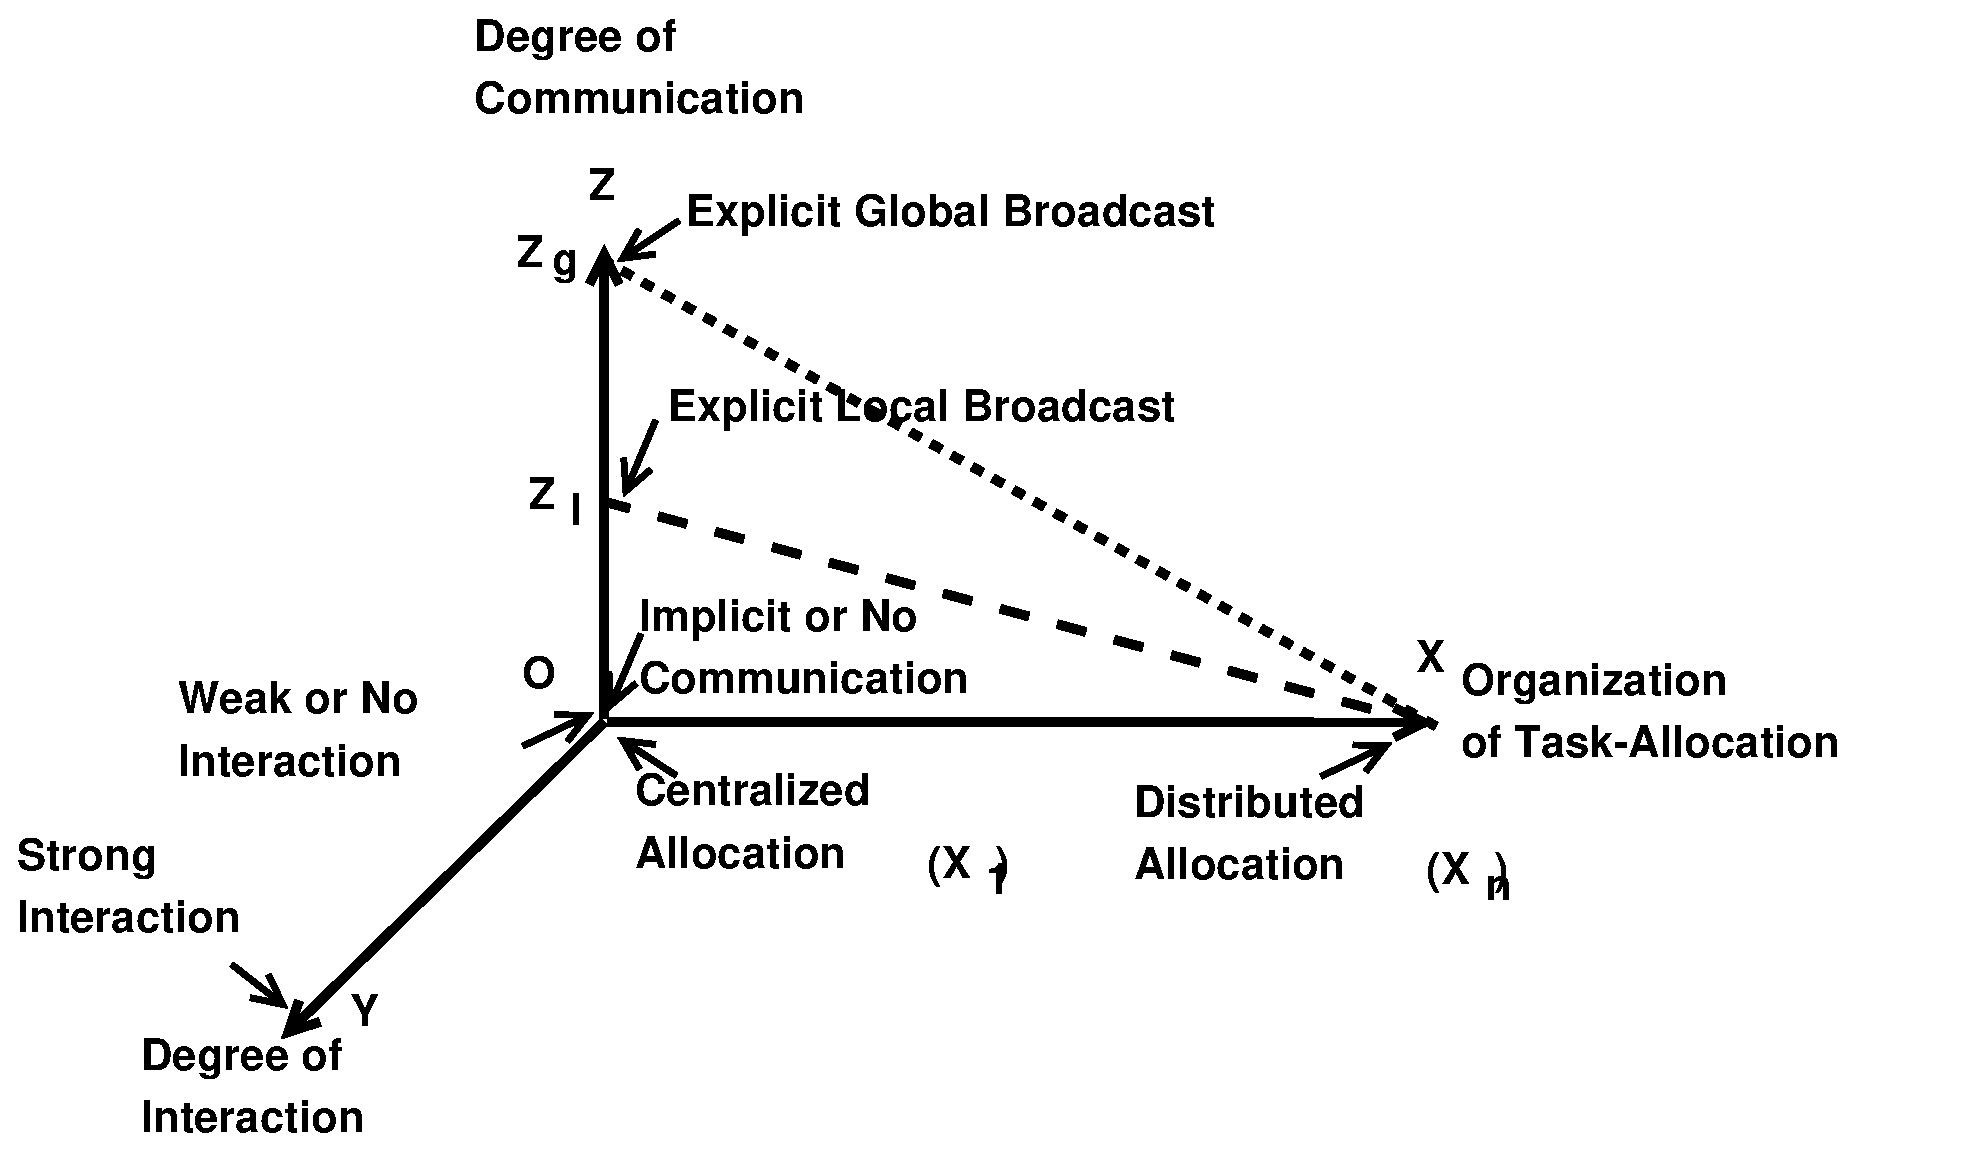
\includegraphics[width=12cm, angle=0]
{./images/mrta-lines.eps}
%figure caption is below the figure
\caption{ Three major axes of complexities in MRTA}
\label{fig:mrta-complexities} % Give a unique label
\end{figure}
%%
In order to characterize both predefined and self-organized approaches in terms of their deployment, we propose three distinct axes: 1) organization of task-allocation (X), 2) degree of interaction (Y) and 2) degree of communication (Z). Fig. \ref{fig:mrta-complexities} depicts these axes with a reference point $O$. These axes can be used to measure the complexities involved in various kinds of MRTA problems and the design of their solutions. 

In Fig. \ref{fig:mrta-complexities}, X axis represents the number of active nodes that provides the task-allocation to the group. For example, in any predefined  task-allocation approach, we can use one external centralized entity or one of the robots (aka leader) to manage the task-allocation. In many predefined methods, e.g. in market-based systems,  multiple nodes can act as mediators or task-allocators that we have discussed before. Under predefined task-allocation approach,  a small number of robots can have fully distributed task-allocation where each robot acts as an independent task-allocator (e.g. as discussed before in ALLIANCE architecture). 

Most of the self-organized task-allocation methods are fully distributed, i.e. they allocate their tasks independently without the help of a centralized entity. However, they might be dependent on external entities for getting status or descriptions of tasks. Recent studies on swarm-robotic flocking by \citet{Celikkanat+2008} show that a swarm can be guided to a target by a few informed individuals (or leaders) while  maintaining the self-organizing principles of task-allocation. Task-allocation of a swarm of robots  just by one central entity may be rare since one of the major spirits of swarm robotic system is to become fully distributed.

In Fig. \ref{fig:mrta-complexities},  Y axis corresponds to the level of robot-robot interaction present in the system. Group-level interaction can be classified into various levels: collective, cooperative, coordinative and collaborative \cite{Parker2008}. The presence of interaction can be due to the nature of the problem, e.g. cooperation is necessary in co-operative transport tasks. Alternately, this interaction can be a design choice where interaction can improves the performance of the team, e.g. cooperation in cleaning a work-site is not necessary but it can help to improve the  efficiency of this task. 

Y axis can also be used to refer to the degree of coupling present in the system.  In case of collective interaction, robots merely co-exist, i.e.  they may not be aware of each other except treating others as obstacles. Many other multi-robot systems are loosely-coupled where robots can indirectly infer some states of the environment from their team-mates' actions.  But in many cases, e.g. in  co-operative transport, robots not only recognize others as their team-mates, but also they coordinate their actions. Thus they form a  tightly coupled system. This level of interaction and coupling also gives us the information about potential side-effects of failure of an individual robot. Tightly coupled systems with high degrees of interactions among the robots  suffer from the performance loss if some of the robots removed from the system.

The Z axis of Fig. \ref{fig:mrta-complexities} represents the communication overhead of the system. This can be the result of the interactions  of robots under a given task-allocation method. As we have discussed before various task-allocation methods rely upon variable degrees of robot-robot communications.  On the other hand, the communication capabilities of individual robots can limit (or expand) the level of interaction can be made  in a given group. Thus in one way, considering the interaction requirements of a MRTA problem, the system designer can  select suitable communication strategies that both minimizes the communication overhead and maximizes the performance of the group. And in other way, the communication capabilities of robots can guide a system designer to design interaction rules of robot teams, e.g. the specification of robot's on-board camera  can determine the degree of possible visual interactions among robots. The suitable trade-offs between these two axes: communication and interaction can give us a balanced design of our MRTA solutions.

The central issue of this paper is to determine the role of communication and sensing strategies under an adaptive response-threshold task-allocation method. So we have focused to examine the benefits of traversing along the various axes of Fig. \ref{fig:mrta-complexities}. In this paper, we are interested on two distinct lines: 1) distributed task-allocation, with no direct robot-robot interaction and communication, say line $OX_{n}$ ($n$ being the number of robots)  and 2) distributed task-allocation, with no direct robot-robot interaction, but varying degrees of local communications, say line $X_{n}Z_{l}$  ($Z_{l}$ being a local broadcast communication strategy that involves $l$ number of peers in communication).
%%============================================================
\section{Robotic interpretation of the Attractive Field Model}
\label{sec:afm}
%%
\section{AFM based task-allocation solution}
\label{sec:mrta}
%%
\section{Experiments}
\label{sec:expt}
%%
\section{Results}
\label{sec:res}
%%
\section{Discussions}
\label{sec:discuss}
%%
\section{Conclusions}
\label{sec:conc}
%% The Appendices part is started with the command \appendix;
%% appendix sections are then done as normal sections
%% \appendix
%% \section{}
%% \label{}
%% References
%%
%% Following citation commands can be used in the body text:
%% Usage of \cite is as follows:
%%   \cite{key}         ==>>  [#]
%%   \cite[chap. 2]{key} ==>> [#, chap. 2]
%%

%% References with bibTeX database:
\bibliographystyle{./elsart/elsarticle-num}
\bibliography{ras1}
%% Authors are advised to submit their bibtex database files. They are
%% requested to list a bibtex style file in the manuscript if they do
%% not want to use elsarticle-num.bst.
%% References without bibTeX database:
% \begin{thebibliography}{00}
%% \bibitem must have the following form:
%%   \bibitem{key}...
%%
% \bibitem{}
% \end{thebibliography}
\end{document}
%%
%% End of file `elsarticle-template-num.tex'.